\section{Conceituação Básica}

\begin{frame}[t, fragile]{Manutenção de Software}
    \begin{block}{Definição:}
    \alert{Modificação} do produto de software \alert{após} a sua colocação em \alert{uso} \textcolor{Blue}{\cite{Sommerville2011}}.
    \end{block}
    
    \begin{figure}[hbt]
    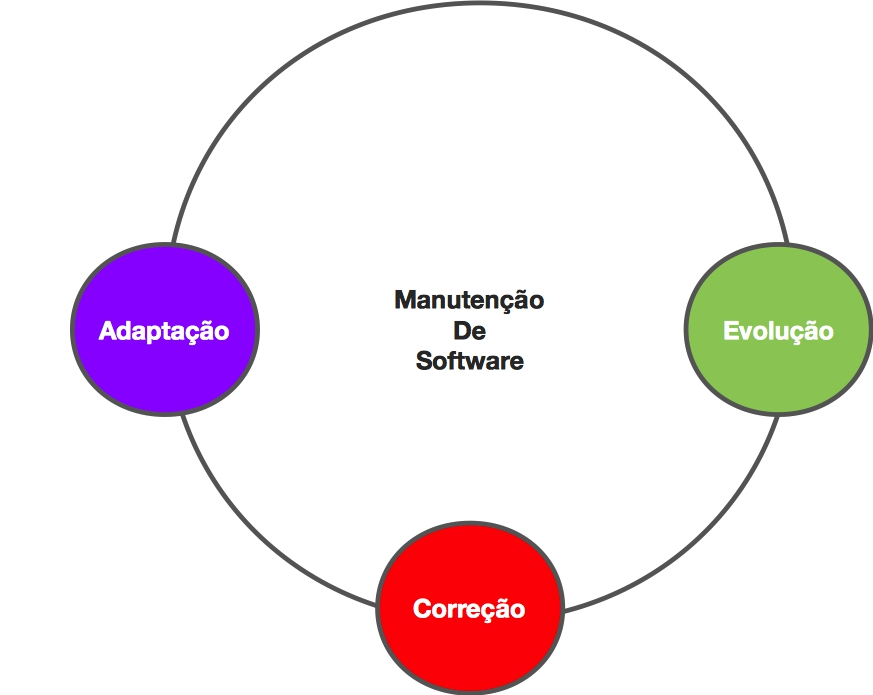
\includegraphics[width=0.5\textwidth]{imagens/tipos-de-manuntencao.jpg}
  \end{figure}
    
\end{frame}

\begin{frame}[t, fragile]{Manutenibilidade}
    \begin{itemize}
      \item \alert{Não} existe um \alert{entendimento} comum sobre o que é \alert{manutenibilidade}, como
        ela pode ser \underline{atingida}, \underline{medida} e \underline{avaliada}
%      \begin{itemize}
%        \item Diferentemente de outros atributos como desempenho
%        \item Toda organização de software de tamanho significativo parece ter a sua própria definição
%        de tamanho
%      \end{itemize}

%      \item O glossário de termos da IEEE define \alert{manutenibilidade} assim:
%      \begin{itemize}
%        \item \textbf{Manutenibilidade} mede a \alert{facilidade} com que o sistema pode ser \alert{modificado} para corrigir falhas, 
%        melhorar o desempenho ou outros atributos, ou adaptar à mudanças no ambiente \textcolor{Blue}{(IEEE)}.
%%      \end{itemize}
%%\framebreak       
%%      \item O Software Engineering Institute define \alert{manutenibilidade} assim:
%%      \begin{itemize}
%        \item \textbf{Manutenibilidade}  \alert{esforço} necessário para realizar \alert{modificações} na \alert{implementação} de um componente específico \textcolor{Blue}{(SEI)}.
%      \end{itemize}
%\framebreak      
%      \item A norma ISO/IEC 9126 define \alert{manuteniblidade} assim:
      %\begin{itemize}
      
  \end{itemize}
  \begin{block}{Definição:}
        \textbf{Manutenibilidade} mede o \alert{esforço} necessário para fazer \alert{modificações} específicas no software \textcolor{Blue}{\cite{Cortes2001}}.
      \end{block}
  
  \begin{figure}[hbt]
    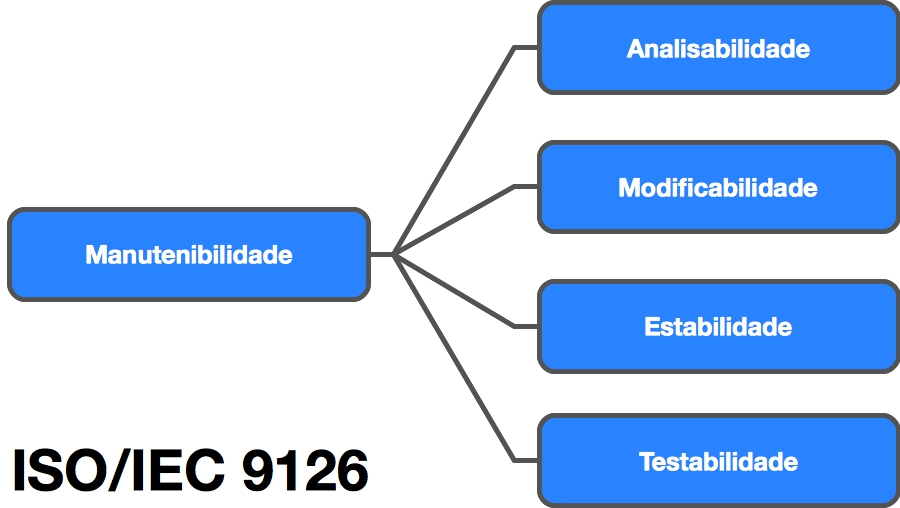
\includegraphics[width=0.5\textwidth]{imagens/subcaracteristica-manutenibilidade.jpg}
  \end{figure}
  
\end{frame}

\begin{frame}[t, fragile]{Índice de Manutenibilidade}
    \begin{block}{Definição:}
      \scriptsize{
      $MI = 171 - 5.2 \times \ln(aveV) - 0.23 \times aveV(g') 
        - 16.2 \times ln(aveLoc) + 50.0 \times \sin \sqrt{2.46 \times perCM}$
      }
    \end{block}
    \textbf{Onde:}
    \begin{tabular}{@{}>{$}l<{$}l@{}}
    aveV & average Halstead Volume\\
    aveV(g') & average extended cyclomatic complexity \\
    aveLoc & average count of lines of code (LOC)\\
    perCM & average percent of lines of comments
  \end{tabular}
       
\end{frame}

%\begin{frame}[allowframebreaks, t, fragile]{Sub-características da Manutenibilidade (ISO/IEC 9126)}
%        \begin{itemize}
%          \item \textbf{Analisabilidade}: medida de esforço necessário para diagnosticar deficiências ou causas de 
%            falhas, ou localizar as partes a serem modificadas para corrigir os problemas
%          \item \textbf{Modificabilidade}: medida de esforço necessário para realizar alterações, remover falhas ou 
%            para adequar o produto a eventuais mudanças de ambientes operacionais
%          \item \textbf{Estabilidade}: medida do risco de efeitos inesperados provenientes de modificações
%          \item \textbf{Testabilidade}: medida de esforço necessário para testar o software alterado
%        \end{itemize}
%
%\end{frame}

\begin{frame}[allowframebreaks, t, fragile]{Linhas de Produtos de Software}
    \begin{block}{Definição:}
        Um \alert{conjunto} de sistema de software que \alert{compartilham} intensivamente um \alert{conjunto comum} e gerenciado de funcionalidades \textcolor{Blue}{\cite{Clements2002}}. 
    \end{block}

    \begin{figure}[hbt]
      
      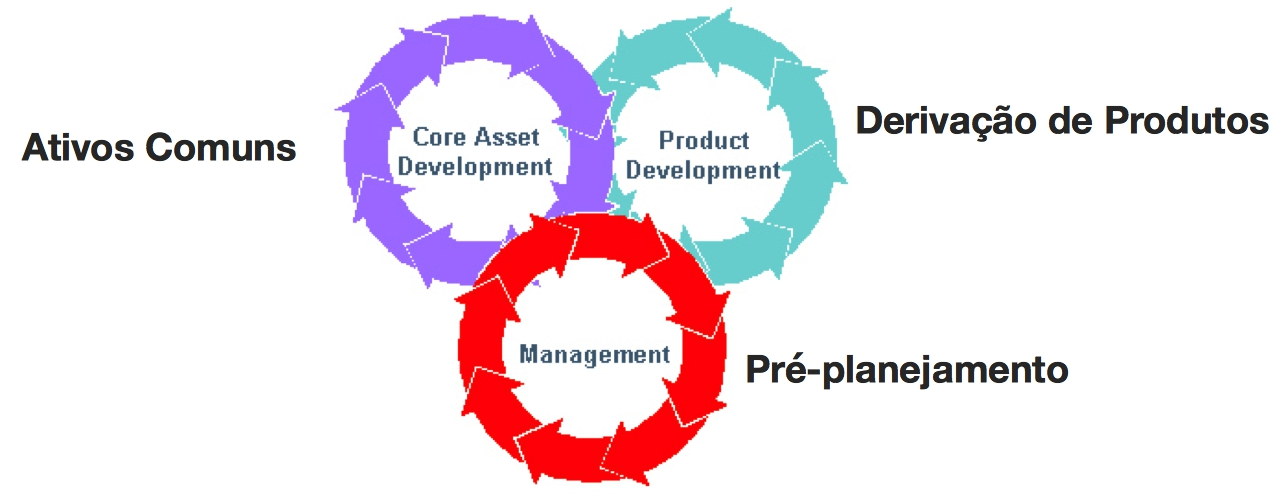
\includegraphics[width=0.8\textwidth]{imagens/atividades-essenciais-1}
      %\caption{Adaptada de \ref{Clements2001}.}
    \end{figure}
\end{frame}

\begin{frame}[allowframebreaks, t, fragile]{Feature Model}
    \begin{itemize}
     \item Feature model é um meio para \alert{representação} de um espaço de \alert{configuração} de todos os produtos de 
     uma \alert{família} de sistemas em termos de suas \textit{features}.
    \end{itemize}
    
    \begin{block}{Definição:}
      Features podem ser definidas como \alert{aspectos}, \alert{qualidades} ou \alert{características} de uma \alert{família} de sistemas.
    \end{block}
    
      \begin{figure}[hbt]
      
      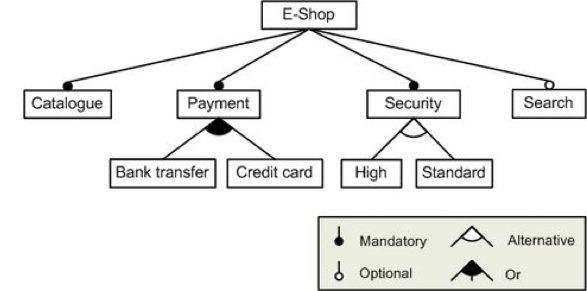
\includegraphics[width=0.8\textwidth]{imagens/exemplo-feature-model-1.jpg}
      %\caption{Adaptada de \ref{Clements2001}.}
    \end{figure}
\end{frame}

% \subsection{Importância}
% \begin{frame}[allowframebreaks, t, fragile]{Por que é Importante ?}
%    \begin{itemize}
%     \item Virtualmente quaisquer organização dependente de software tem vital interesse na redução das suas 
%       atividades de manutenção
%     
%     \item Manutenibilidade é amplamente aceita como um importante atributo de qualidade de sistemas de software
%       em razão do seu impacto econômico.
%       
%     \item Manutenibilidade de software tornou-se uma das mais importantes preocupações da indústria de software
%     \item F.Brooks reivindica "O custo total de manter um software é tipicamente 40 porcento ou mais do custo de desenvolvimento"
% 
%     \item Parik tem uma visão mais pessimista, reivindicando que de 45 a 60 é gasto com manutenção".
%     \item Corbi and Yourdon reivindica que a manutenibilidade de software e um dos maiores desafios para da década de 1990
%     
%    \end{itemize}
% \end{frame}
% 
% \subsection{Modelos de Avaliação da Manutenibilidade}
% \begin{frame}[allowframebreaks, t, fragile]{Modelos de Avaliação da Manutenibilidade}
%    \begin{itemize}
%     \item \textbf{Modelo de avaliação multidimensional}:   
%     \item \textbf{Modelo de regressão polinominal}: 
%     \begin{itemize}
%       \item Explora o relacionamento entre a manutenibilidade de software e as métricas de software. 
%     \end{itemize}   
%     \item \item \textbf{Medida de agregação de complexidade}:
%     \item \textbf{Análise de componentes principais}:
%     \item \textbf{Análise de fator}
%    \end{itemize}
% \end{frame}
% 
% \subsection{Manutenção versus Manutenibilidade}
% \begin{frame}[t, fragile]{Manutenção versus Manutenibilidade}
%     blabla
% \end{frame}
